\label{sec:pilot-data-hadoop}
Our approach is to design a common software environment while attempting to be agnostic of specific hardware infrastructures, technologies and trends.
In this section, we provide background information and comparative information on system abstractions, resource management and interoperability in HPC and Hadoop.

Hadoop~\cite{hadoop} has evolved to become the standard implementation of the MapReduce abstraction on top of the Hadoop filesystem and the YARN resource management.
In fact, over the past years, Hadoop evolved to a general purpose cluster computing framework suited for data-intensive applications in industry~\cite{luckow2015automotive} and sciences~\cite{jha2014tale}.

HPC and Hadoop originated from the need to support different kinds of applications: compute-intensive applications in the case of HPC, and data-intensive in the case of Hadoop.
Not surprisingly, they follow different design paradigms: In HPC environments, storage and compute are connected by a high-end network (e.\,g.\ Infiniband) with capabilities such as RDMA; Hadoop co-locates both.
HPC infrastructures introduced parallel filesystems, such as Lustre, PVFS or GPFS, to meet the increased I/O demands of data-intensive applications and archival storage and to address the need for retaining large volumes of primary simulation output data.
The parallel filesystem model of using large, optimized storage clusters exposing a POSIX compliant rich interface and connecting it to compute nodes via fast interconnects works well for compute-bound task.
It has however, some limitations for data-intensive, I/O-bound workloads that require a high sequential read/write performance.
Various approaches for integrating parallel filesystems, such as Lustre and PVFS, with Hadoop emerged~\cite{kulkarni2013hadoop,tantisiriroj2011duality}, which yielded good results in particular for medium-sized workloads.

While Hadoop simplified the processing of vast volumes of data, it has limitations in its expressiveness as pointed out by various authors~\cite{yelick2011magellan,isard2007dryad}.
The complexity of creating sophisticated applications such as iterative machine learning algorithms required multiple MapReduce jobs and persistence to HDFS after each iteration.
This is lead to several higher-level abstractions for implementing sophisticated data pipelines.
Examples of such higher-level execution management frameworks for Hadoop are: Spark~\cite{zaharia2010spark}, Apache Flink~\cite{flink}, Apache Crunch~\cite{crunch} and Cascading~\cite{cascading}.

The most well-known emerging processing framework in the Hadoop ecosystem is Spark~\cite{zaharia2010spark}.
In contrast to MapReduce, it provides a richer API, more language bindings and a novel memory-centric processing engines, that can utilize distributed memory and can retain resources across multiple task generation.
Spark's \emph{Reliable Distributed Dataset (RDD)} abstraction provides a powerful way to manipulate distributed collection stored in the memory of the cluster nodes.
Spark is increasingly used for building complex data workflows and advanced analytic tools, such as MLLib~\cite{mllib} and SparkR.

Although the addition/development of new and higher-level execution frameworks addressed some of the problems of data processing, it introduced the problem of heterogeneity of access and resource management, which we now discuss.

Hadoop originally provided a rudimentary resource management system, the YARN scheduler~\cite{vavilapalli2013apache} provides a robust application-level scheduler framework addressing the increased requirements with respect to applications and infrastructure: more complex data localities (memory, SSDs, disk, rack, datacenter), long-lived services, periodic jobs, interactive and batch jobs need to be supported on the same environment.
In contrast, to traditional batch schedulers, YARN is optimized for data-intensive environments supporting data-locality and the management of a large number of fine-granular tasks (found in data-parallel applications).

While YARN manages system-level resources, applications and runtimes have to implement an application-level scheduler that optimizes their specific resource requirements, e.\,g.\ with respect to data locality. This application-level scheduler is referred to as {\it Application Master} and is responsible for allocating resources -- the so called containers -- for the applications and to execute tasks in these containers.
Data locality, e.\,g.\ between HDFS blocks and container locations, need to managed by the Application Master by requesting containers on specific nodes/racks.

Managing resources on top of YARN is associated with several challenge: while fine-grained, short-running tasks as found in data-parallel MapReduce applications are well supported, other workload characteristics are less well supported, e.\,g.\ gang-scheduled parallel MPI applications and long-running applications found predominantly in HPC environments.
To achieve interoperability and integration between Hadoop and HPC, it is essential to consider a more diverse set of workloads on top of  YARN.

To achieve interoperability, several frameworks explore the usage of Hadoop on HPC resources.
Various frameworks for running Hadoop on HPC emerged, e.\,g., Hadoop on Demand~\cite{hod}, JUMMP~\cite{moody2013jummp}, MagPie~\cite{chu2015magpie}, MyHadoop~\cite{krishnan2011myhadoop}, MyCray~\cite{mycray}.
While these frameworks can spawn and manage Hadoop clusters many challenges with respect to optimizing configurations and resource usage including the use of available SSDs for the shuffle phase, of parallel filesystems and of high-end network features, e.\,g.\ RDMA~\cite{rahman2014homr} remain.
Further, these approaches do not address the need for interoperability between HPC and Hadoop application stages.

A particular challenge for Hadoop on HPC deployment is the choice of storage and filesystem backend.
Typically, for Hadoop local storage is preferred; nevertheless, in some cases, e.\,g.\ if many small files need to processed, random data access is required or the number of parallel tasks is low to medium, the usage of Lustre or another parallel filesystem can yield in a better performance.
For this purpose, many parallel filesystems provide a special client library, which improves the interoperability with Hadoop; it limits however data locality and the ability for the application to optimize for data placements since applications are commonly not aware of the complex storage hierarchy.
Another interesting usage mode is the use of Hadoop as active archival storage -- in particular, the newly added HDFS heterogeneous storage support is suitable for supporting this use case.

Another challenge is the integration between both HPC and Hadoop environments.
Rather than preserving HPC and Hadoop ``environments'' as software silos, there is a need for an approach that integrates them. 
We propose the Pilot-Abstraction as unifying concept to efficiently support the integration, and not just the interoperability between HPC and Hadoop.
By utilizing the multi-level scheduling capabilities of YARN, Pilot-Abstraction can efficiently manage Hadoop cluster resources providing the application with the necessary means to reason about data and compute resources and allocation.
On the other side, we show, how the Pilot-Abstraction can be used to manage Hadoop applications on HPC environments.

The Pilot-Abstraction~\cite{luckow2012pstar} has been successfully used in HPC environments for supporting a diverse set of task-based workloads on distributed resources.
A Pilot-job is a placeholder job that is submitted to the resource management system representing a container for a dynamically determined set of compute tasks.
Pilot-jobs are a well-known example of multi-level scheduling, which is often used to separate system-level resource and user-level workload management.
The Pilot-Abstraction defines the following entities: A Pilot-Compute allocates a set of computational resources (e.\,g.\,cores); a Compute-Unit (CU) as a self-contained piece of work represented as executable that is submitted to the Pilot-job.
A CU can have data dependencies, i.\,e.\ a set of files that need to be available when executing the CU.
A workloads typically consists of a set of dependents CUs.
The Pilot-Abstraction has been implemented within BigJob~\cite{luckow2012pstar,luckow2010saga} and its second generation prototype RADICAL-Pilot~\cite{merzky2018design}.
The interoperability layer of both frameworks is SAGA~\cite{merzky2015saga}, which is used for accessing the resource management system (e.\,g.\ SLURM, Torque and SGE) and for file transfers.
SAGA is a lightweight interface that provides standards-based interoperable capabilities to the most commonly used functionalities required to develop distributed applications, tools and services.


\subsection{Some title here}
\label{ssec:some_title}
An important motivation of our work is to provide advanced and scalable data analysis capabilities for existing high-performance applications (e.g., large-scale molecular dynamics simulations).
This requires adding data-intensive analysis while preserving high-performance computing capabilities.
Having established the potential of the Pilot~-Abstraction for a range of high-performance applications~\cite{treikalis2016repex,ragothaman2014developing,ko2014numerical}, we use it as the starting point for integrated high-performance compute and data-intensive analysis.
We propose several extensions to RADICAL~-Pilot to facilitate the integrated use of HPC and Hadoop frameworks using the Pilot~-Abstraction.

\begin{figure}[t]
    \centering
    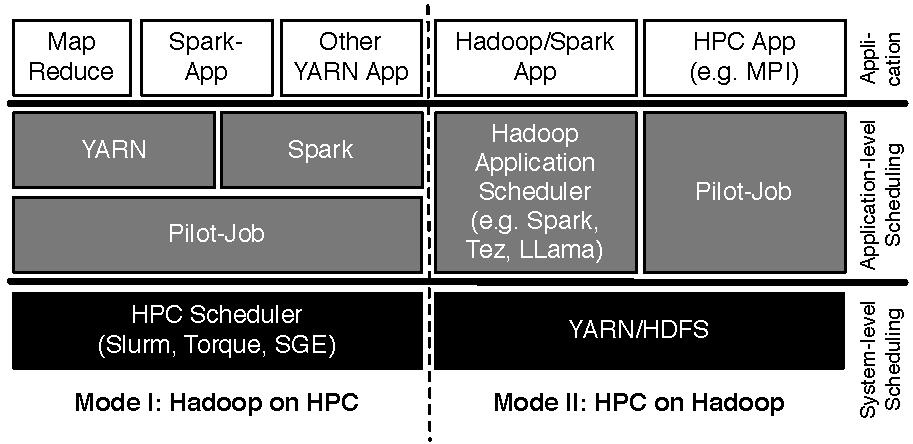
\includegraphics[width=.95\textwidth]{figures/data_analytics_hpc/hpc_hadoop/hadoop-on-hpc-viceverse.pdf}
    \caption{\textbf{Hadoop and HPC Interoperability:}
        There are two usage modes:
        (i) spawning a YARN or Spark cluster on a HPC environment (Hadoop on HPC), and
        (ii) Running HPC applications inside a YARN cluster (HPC on Hadoop).
        \label{fig:figures_hadoop-on-hpc-viceverse}}
\end{figure}

As depicted in Figure~\ref{fig:figures_hadoop-on-hpc-viceverse}, there are at least two different usage modes to consider:
\begin{compactenum}[(i)]
    \item Mode I: Running Hadoop/Spark applications on HPC environments (Hadoop on HPC),
    \item Mode II: Running HPC applications on YARN clusters (HPC on Hadoop).
\end{compactenum}

Mode I is critical to support traditional HPC environments (e.\,g., the majority of XSEDE resources) so as to support applications with both compute and data requirements.
Mode II is important for cloud environments (e.\,g.\ Amazon's Elastic MapReduce, Microsoft's HDInsight) and an emerging class of HPC machines with new architectures and usage modes, such as Wrangler~\cite{wrangler} that support Hadoop natively.
For example, Wrangler supports dedicated Hadoop environments (based on Cloudera Hadoop 5.3) via a reservation mechanism.

In the following we propose a set of tools for supporting both of these usage modes:
In section~\ref{sssec:saga_hadoop} we present SAGA-Hadoop, a light-weight, easy-to-use tool for running Hadoop on HPC (Mode I).
We then discuss, the integration of Hadoop and Spark runtimes into RADICAL~-Pilot, which enables both the interoperable use of HPC and Hadoop, as well as the integration of HPC and Hadoop applications (Mode I and II) (Section~\ref{sssec:rp-impl} to~\ref{sssec:rp_spark}).
Using these new capabilities, applications can seamlessly connect HPC stages (e.\,g.\ simulation stages) with analysis staging using the Pilot-Abstraction to provide unified resource management.

\subsubsection{SAGA-Hadoop: Supporting Hadoop/Spark on HPC}
\label{sssec:saga_hadoop}

SAGA-Hadoop~\cite{saga-hadoop} is a tool for supporting the deployment of Hadoop and Spark on HPC resources (Mode I in Figure~\ref{fig:figures_hadoop-on-hpc-viceverse}).
Using SAGA-Hadoop an applications written for YARN (e.\,g.\ MapReduce) or Spark (e.\,g. PySpark, DataFrame and MLlib applications) can be executed on HPC resources.


Figure~\ref{fig:saga-hadoop} illustrates the architecture of SAGA-Hadoop.
SAGA-Hadoop uses SAGA~\cite{merzky2015saga} to spawn and control Hadoop clusters inside an environment managed by an HPC scheduler, such as PBS, SLURM or SGE, or clouds.
SAGA is used for dispatching a bootstrap process that generates the necessary configuration files and for starting the Hadoop processes.
The specifics of the Hadoop framework (i.\,e.\ YARN and Spark) are encapsulated in a Hadoop framework plugin (also commonly referred to as adaptors).
SAGA-Hadoop delegates tasks, such as the download, configuration and start of a framework to this plugin.
In the case of YARN, the plugin is then responsible for launching YARN's Resource and Node Manager processes; in the case of Spark, the Master and Worker processes.
This architecture allows for extensibility -- new frameworks, e.\,g.\ Flink, can easily be added.


While nearly all Hadoop frameworks (e.\,g.\ MapReduce and Spark) support YARN for resource management, Spark provides a standalone cluster mode, which is more efficient in particular on dedicated resources.
Thus, a special adaptor for Spark is provided.
Once the cluster is setup, users can submit applications using a simple API that allows them to start and manage YARN or Spark application processes.

\begin{figure}[t]
    \centering
    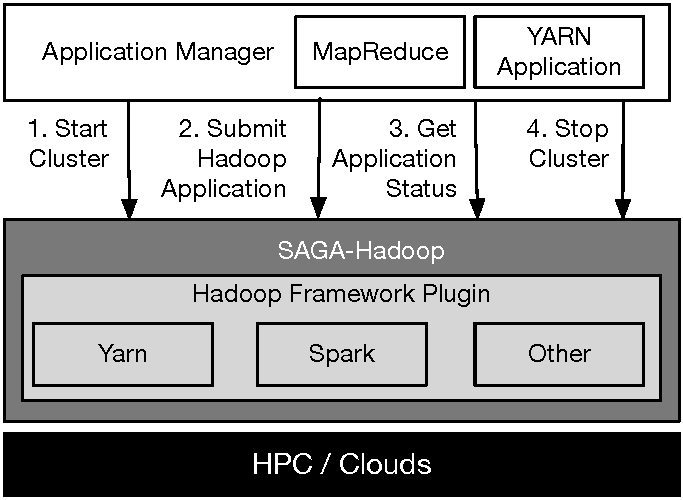
\includegraphics[width=.95\textwidth]{figures/data_analytics_hpc/hpc_hadoop/pilot-abds.pdf}
    \caption{\textbf{SAGA-Hadoop for HPC and Cloud Infrastructures:} 
        SAGA-Hadoop provides  uniform framework to managing Hadoop and Spark clusters on resources managed by HPC schedulers, such as PBS, SGE and SLURM.}
    \label{fig:saga-hadoop}
\end{figure}

While SAGA-Hadoop provides the interoperability between YARN and HPC resources by treating YARN as a substitute for SLURM or Torque, the integration of YARN and HPC application or application stages remains challenging.
In the following, we explore the usage of the Pilot~-Abstraction, an implementation of which is RADICAL~-Pilot, to enable the integration between these different application types.

\subsubsection{RADICAL~-Pilot and YARN Overview}
\label{sssec:rp-impl}


With the introduction of YARN, a broader set of applications can be executed within Hadoop clusters than earlier.
However, developing and deploying YARN applications potentially side-by-side with HPC applications remains a difficult task.
Established abstractions that are easy-to-use while enabling the user to reason about compute and data resources across infrastructure types (i.\,e.\ Hadoop, HPC and clouds) are missing. 

Schedulers such as YARN effectively facilitate application-level scheduling, the development efforts for YARN applications are high. YARN provides a low-level abstraction for resource management, e.g., a Java API and protocol buffer specification.
Typically interactions between YARN and the applications are much more complex than the interactions between an application and a HPC scheduler.
Further, applications must be able to run on a dynamic set of resources; YARN e.\,g.\ can preempt containers in high-load situations.
Data/compute locality need to be manually managed by the application scheduler by requesting resources at the location of an file chunk.
Also, allocated resources (the so called YARN containers) can be preempted by the scheduler.

To address these shortcomings, various frameworks that aid the development of YARN applications have been proposed: Llama~\cite{llama} offers a long-running application master for YARN designed for the Impala SQL engine.
Apache Slider~\cite{apache-slider} supports long-running distributed application on YARN with dynamic resource needs allowing applications to scale to additional containers on demand.
While these frameworks simplify development, they do not address concerns such as interoperability and integration of HPC/Hadoop.
In the following, we explore the integration of YARN into the RADICAL~-Pilot (RP) framework.
This approach allows applications to run HPC and YARN application parts side-by-side.

% RADICAL-Pilot Overview
Figure~\ref{fig:comp_rp_arch} illustrates the architecture of RADICAL~-Pilot and the components that were extended for YARN.
The figure on the left shows the macro architecture of RADICAL~-Pilot; the figure on the right a blown-up look into the architecture of the Pilot-Agent which is a critical functional component.
RADICAL~-Pilot consists of a client module with the Pilot-Manager and Unit-Manager and a set of RADICAL~-Pilot-Agents running on the resource.
The Pilot-Manager is the central entity responsible for managing the lifecycle of a set of Pilots: Pilots are described using a Pilot description, which contains the resource requirements of the Pilot and is submitted to the Pilot-Manager.
The Pilot-Manager submits the placeholder job that will run the RADICAL~-Pilot-Agent via the Resource Management System using the SAGA-API (steps P.1-P.7).
Subsequently, the application workload (the Compute-Units) is managed by the Unit-Manager and the RADICAL~-Pilot-Agent (steps U.1-U.7).
More details are available at~\cite{merzky2019using}.

\begin{figure*}
    \centering
    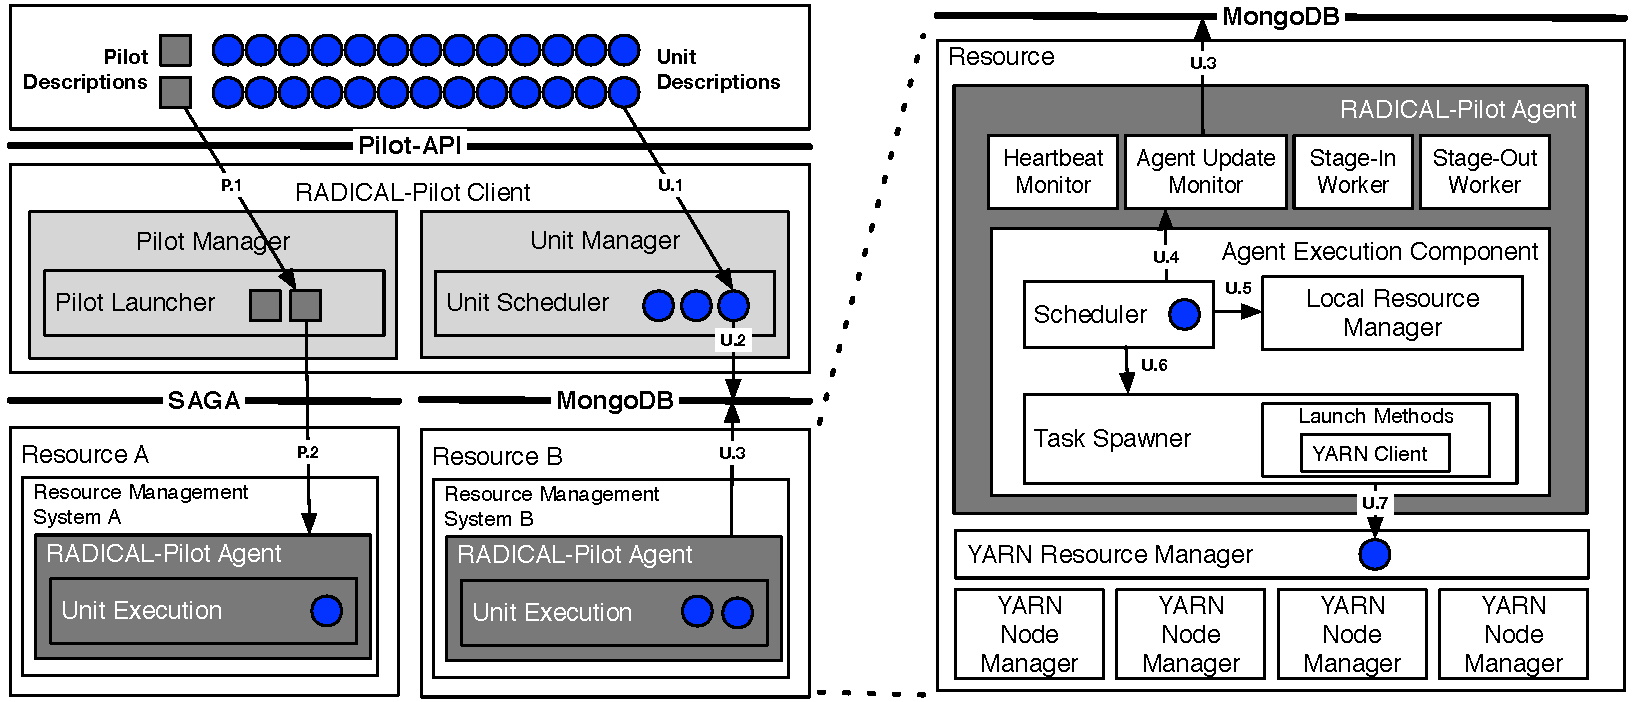
\includegraphics[width=0.95\textwidth]{figures/data_analytics_hpc/hpc_hadoop/rp-architecture-yarn.pdf}
    \caption{\textbf{RADICAL-Pilot and YARN Integration:}
        There are two main interactions between the application and RADICAL~-Pilot -- the management of Pilots (P.1-P.2) and the management of Compute Units (U.1-U.7).
        All YARN specifics are encapsulated in the RADICAL-Pilot-Agent.\label{fig:comp_rp_arch}}
\end{figure*}

The RADICAL~-Pilot-Agent has a modular and extensible architecture and consists of the following components: the Agent Execution Component, the Heartbeat Monitor, Agent Update Monitor, Stage In and Stage Out Workers.
The main integration of YARN and RP is done in the Agent Execution Component.
This component consist of four sub-components:
The {\bf scheduler} is responsible for monitoring the resource usage and assigning CPUs to a Compute Units.
The {\bf Local Resource Manager} (LRM) interacts with the batch system and communicates to the Pilot and Unit Managers the number of cores it has available and how they are distributed.
The {\bf Task Spawner} configures the execution environment, executes and monitors each unit.
The {\bf Launch Method} encapsulates the environment specifics for executing an applications, e.\,g.\ the usage of \texttt{mpiexec} for MPI applications, machine-specific launch methods (e.g. \texttt{aprun} on Cray machines) or the usage of YARN.
After the Task Spawner completes the execution of a unit, it collects the exit code, standard input and output, and instructs the scheduler about the freed cores.


\subsubsection{Integration of RADICAL~-Pilot and YARN}
\label{sssec:rp-yarn}

There are two integration options for RADICAL~-Pilot and YARN: (i) Integration on Pilot-Manager level, via a SAGA adaptor, and (ii) integration on the RADICAL~-Pilot-Agent level.
The first approach is associated with several challenges: firewalls typically prevent the communication between external machines and a YARN clusters.
A YARN application is not only required to communicate with the resource manager, but also with the node managers and containers; further, this approach would require significant extension to the Pilot-Manager, which currently relies on the SAGA Job API for launching and managing Pilots.
Capabilities like the on-demand provisioning of a YARN cluster and the complex application-resource management protocol required by YARN are difficult to abstract behind the SAGA API.  

The second approach encapsulated YARN specifics on resource-level.
If required, a YARN cluster is de-centrally provisioned.
Units are scheduled and submitted to the YARN cluster via the Unit-Manager, the MongoDB-based communication protocol and the RADICAL~-Pilot-Agent scheduler.
By integrating at the RADICAL~-Pilot-Agent level, RADICAL~-Pilot supports both Mode I and II as outlined in Figure~\ref{fig:figures_hadoop-on-hpc-viceverse}.

As illustrated in Figure~\ref{fig:comp_rp_arch}, in the first phase (step P.1 and P.2) the RADICAL~-Pilot-Agent is started on the remote resource using SAGA, e.\,g.\ SLURM.
In Mode I, during the launch of the RADICAL~-Pilot-Agent the YARN cluster is spawned on the allocated resources (Hadoop on HPC); in Mode II the RADICAL~-Pilot-Agent will just connect to a YARN cluster running on the machine of the RADICAL~-Pilot-Agent.
Once the RADICAL~-Pilot-Agent has been started, it is ready to accept Compute Units submitted via the Unit-Manager (step U.1).
The Unit-Manager queues new Compute Units using a shared MongoDB instance (step U.2).
The RADICAL~-Pilot-Agent periodically checks for new Compute Units (U.3) and queues them inside the scheduler (U.4).
The execution of the Compute Unit is managed by the Task Spawner (step U.6 and U.7).
In the following, we describe how these components have been extended to support YARN.


The \emph{Local Resource Manager (LRM)} provides an abstraction to local resource details for other components of the RADICAL~-Pilot-Agent.
The LRM evaluates the environment variables provided by the resource management systems to obtain information, such as the number of cores per node, memory and the assigned nodes.
This information can be accessed through the Resource Manager's REST API.
As described, there are two deployment modes.
In Mode I (Hadoop on HPC), during the initialization of the RADICAL~-Pilot-Agent, the LRM setups the HDFS and YARN daemons: 
First, the LRM downloads Hadoop and creates the necessary configuration files, i.\,e. the \texttt{mapred-site.xml}, \texttt{core-site.xml}, \texttt{hdfs-site.xml}, \texttt{yarn-site.xml} and the slaves and master file containing the allocated nodes.
The node that is running the Agent are assigned to run the master daemons: the HDFS Namenode and the YARN Resource Manager.
After the configuration files are written, HDFS and YARN are started and meta-data about the cluster, i.\,e.\ the number of cores and memory, are provided to the scheduler.
They remain active until all the tasks are executed.
Before termination of the agent, the LRM stops the Hadoop and YARN daemons and removes the associated data files.
In Mode II (Hadoop on HPC), the LRM solely collects the cluster resource information.

The \emph{scheduler} is another extensible component of the RADICAL~-Pilot-Agent responsible for queueing compute units and assigning these to resources.
For YARN we utilize a special scheduler that utilizes updated cluster state information (e.\,g.\ the amount of available virtual cores, memory, queue information, application quotas etc.) obtained via the Resource Manager's REST API.
In contrast to other RADICAL~-Pilot schedulers, it specifically utilizes memory in addition to cores for assigning resource slots.

\emph{Task Spawner and Launch Method:}
The Task Spawner is responsible for managing and monitoring the execution of a Compute Unit.
The Launch Method components encapsulates resource/launch-method specific operations, e.\,g.\ the usage of the \texttt{yarn} command line tool for submitting and monitoring applications.
After launch of a Compute Unit, the Task Spawner periodically monitors its execution and updates its state in the shared MongoDB instance.
For YARN the application log file is used for this purpose.

\begin{figure}[t]
    \centering
    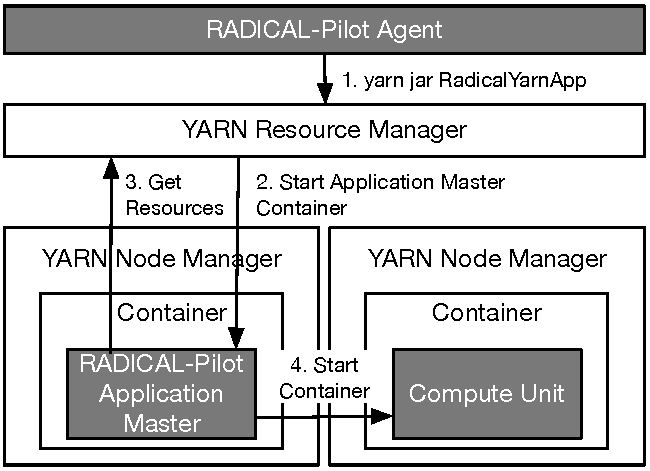
\includegraphics[width=.95\textwidth]{figures/data_analytics_hpc/hpc_hadoop/yarn.pdf}
    \caption{\textbf{RADICAL~-Pilot YARN Agent Application: }
        RADICAL~-Pilot provides a YARN application that manages the execution of Compute Units.
        The application is initialized with parameters defined in the Compute Unit Description and started by the Task Spawner (step 1/2).
        The Application Master requests resources from the Resource Manager and starts a container running the Compute Unit (step 3/4).}
    \label{fig:figures_yarn}
\end{figure}

\emph{RADICAL~-Pilot Application Master:}
A particular integration challenge is the multi-step resource allocation process imposed by YARN depicted in Figure~\ref{fig:figures_yarn}, which differs significantly from HPC schedulers.
The central component of a YARN application is the Application Master, which is responsible for negotiating resources with the YARN Resource Manager as well as for managing the execution of the application in the assigned resources.
The unit of allocation in YARN is a so called container (see~\cite{murthy2014apache}).
The YARN client (part of the YARN Launch Method) implements a so-called YARN Application Master, which is the central instance for managing the resource demands of the application.
RADICAL~-Pilot utilizes a managed application master that is run inside a YARN container.
Once the Application Master container is started, it is responsible for subsequent resource requests; in the next step it will request the a YARN container meeting the resource requirements of the Compute Unit from the Resource Manager.
Once a container is allocated by YARN, the CU will be started inside these containers.
A wrapper script responsible for setting up a RADICAL~-Pilot environment, staging of the specified files and running the executable defined in the Compute Unit Description is used for this purpose.
Every Compute Unit is mapped to a YARN application consisting of an Application Master and a container of the size specified in the Compute Unit Description.
In the future, we will further optimize the implementation by providing support for Application Master and container re-use.


\subsubsection{Spark Integration}
\label{sssec:rp_spark}
Spark offers multiple deployment modes: standalone, YARN and Mesos.
While it is possible to support Spark on top of YARN, this approach is associated with significant complexity and overhead as two instead of one framework need to be configured and run.
Since we RADICAL~-Pilot operates in user-space and single-user mode, no advantages with respect to using a multi-tenant YARN cluster environment exit.
Thus, we decided to support Spark via the standalone deployment mode.

Similar to the YARN integration, the necessary changes for Spark are confined to the RADICAL~-Pilot-Agent.
Similarly, the Local Resource Manager is mainly responsible for initialization and deployment of the Apache Spark environment.
In the first step the LRM detects the number of cores, memory and nodes provided by the Resource Management System, verifies and downloads necessary dependencies (e.\,g.\ Java, Scala, and the necessary Spark binaries).

It then creates the necessary configuration files, e.\,g.\ \texttt{spark-env.sh}, \texttt{slaves} and \texttt{master} files, required for running a multi-node, standalone Spark cluster.

Finally, the LRM is starting the Spark cluster using the previously generated configuration.
Similar to YARN, a Spark RADICAL~-Pilot-Agent scheduler is used for managing Spark resource slots and assigning CUs.
During the termination of the RADICAL~-Pilot-Agent, the LRM is shutting down the Spark cluster using Spark’s \texttt{sbin/stop-all.sh} script, which stops both the master and the slave nodes.
Similarly, the Spark specific methods for launching and managing Compute Units on Spark are encapsulated in a Task Spawner and Launch Method component.

\subsection{Experiments and Evaluation}
\label{ssec:rph-exps}

To evaluate the RADICAL~-Pilot YARN and Spark extension, we conduct two experiments: in Section~\ref{sec:startup_pilot_unit}, we analyze and compare RADICAL~-Pilot and RADICAL~-Pilot-YARN with respect to startup times of both the Pilot and the Compute Units.
We use the well-known K-Means algorithm to investigate the performance and runtime trade-offs of a typical data-intensive application.
Experiments are performed on two different XSEDE allocated machines: Wrangler~\cite{wrangler} and Stampede~\cite{stampede}.
On Stampede every node has 16 cores and 32 GB of memory; on Wrangler 48\,cores and 128\,GB of memory.

\subsubsection{Pilot Startup and Compute Unit Submission}
\label{sssec:startup_pilot_unit}

\begin{figure}
    \centering
    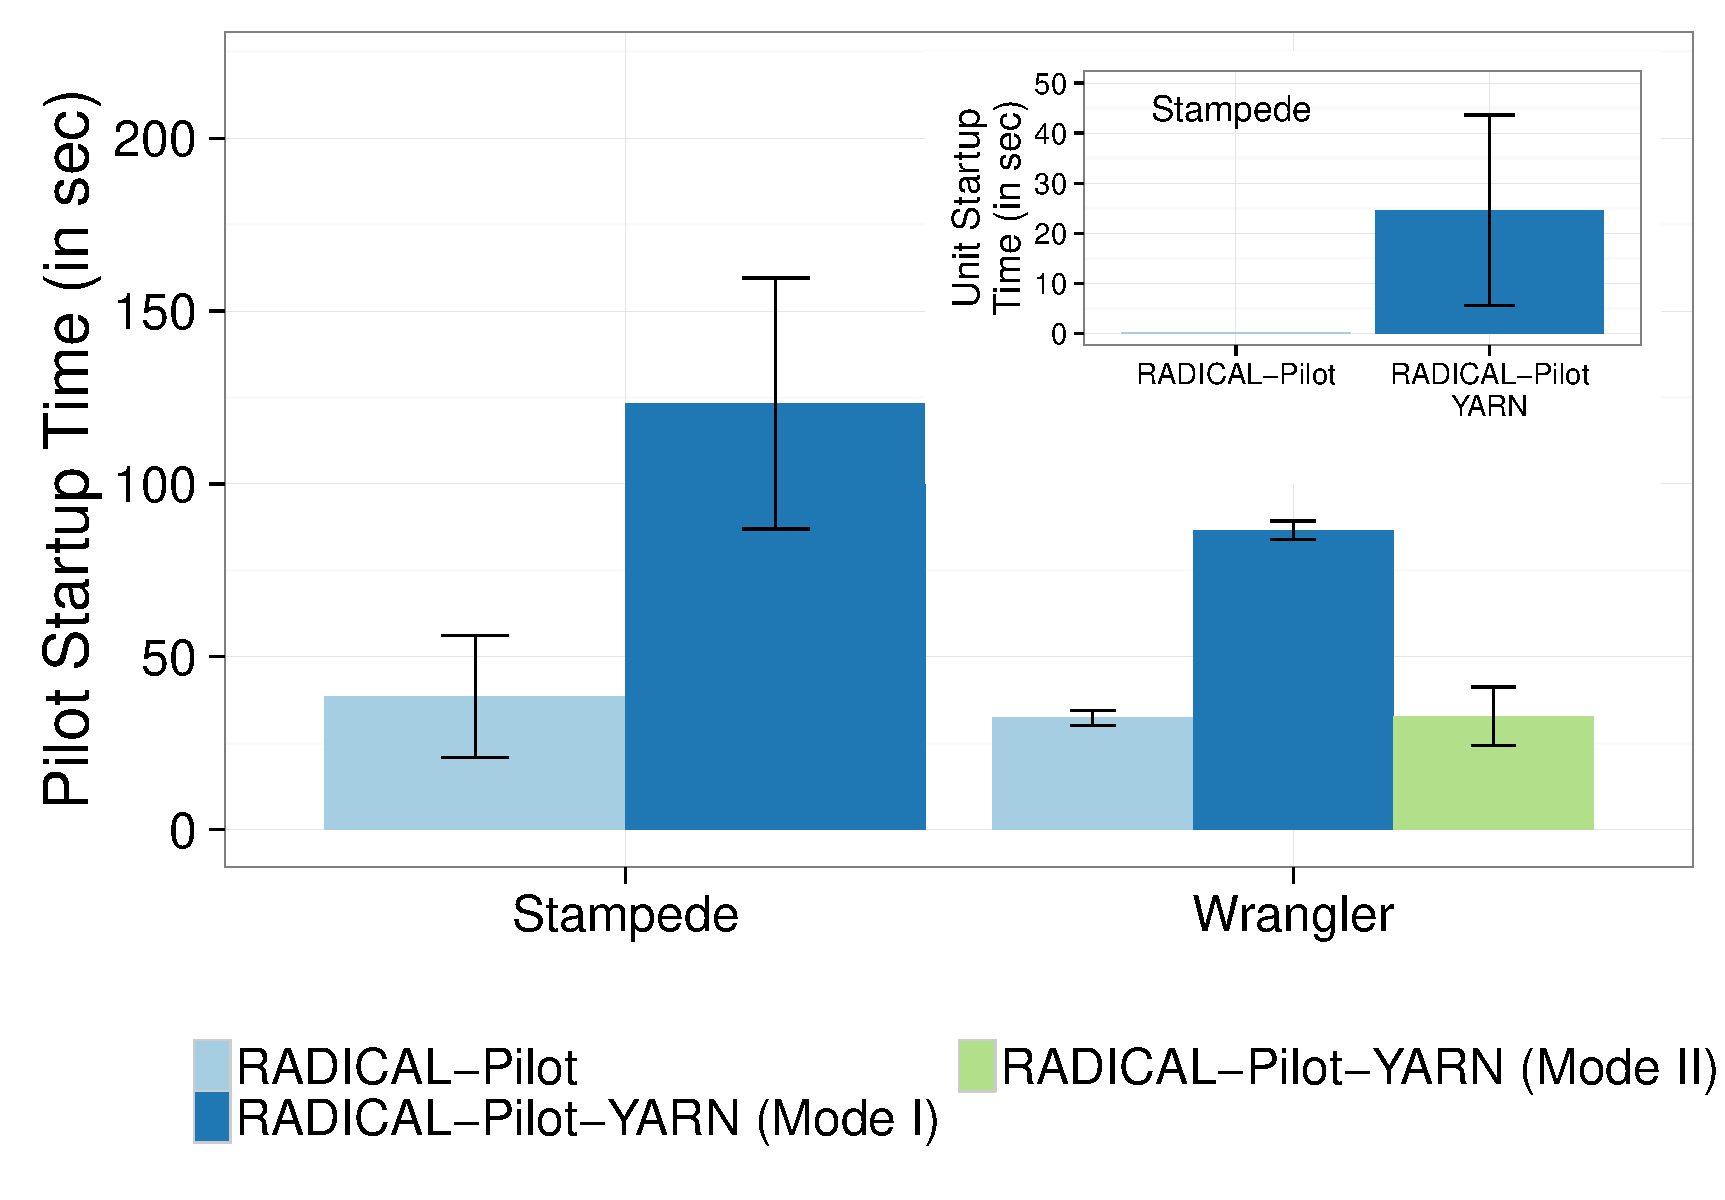
\includegraphics[width=0.85\textwidth]{figures/data_analytics_hpc/hpc_hadoop/pilot_unit_startup.pdf}
    \caption{\textbf{RADICAL~-Pilot and RADICAL~-Pilot-YARN Overheads:}
        The agent startup time is higher for YARN due to the overhead for spawning the YARN cluster.
        The inset shows that the Compute Unit startup time (time between application submission to YARN and startup) is also significantly higher for YARN.
        \label{fig:startup_yarn}}
\end{figure}

In Figure~\ref{fig:startup_yarn} we analyze the measured overheads when starting RADICAL~-Pilot and RADICAL~-Pilot-YARN, and when submitting Compute Units.
The agent startup time for RADICAL~-Pilot-YARN is defined as the time between RADICAL~-Pilot-Agent start and the processing of the first Compute Unit.
On Wrangler, we compare both Mode I (Hadoop on HPC) and Mode II (HPC on Hadoop).
For Mode I the startup time is higher compared to the normal RADICAL~-Pilot startup time and also compared to Mode II.
This can be explained by the necessary steps required for download, configuration and start of the YARN cluster.
For a single node YARN environment, the overhead for Mode I (Hadoop on HPC) is between 50-85\,sec depending upon the resource selected.
The startup times for Mode II on Wrangler -- using the dedicated Hadoop environment provided via the data portal -- are comparable to the normal RADICAL~-Pilot startup times as it is not necessary to spawn a Hadoop cluster.

The inset of Figure~\ref{fig:startup_yarn} shows the time taken to start Compute Units via RADICAL~-Pilot to a YARN cluster.
For each CU, resources have to be requested in two stages: first the application master container is allocated followed by the containers for the actual compute tasks.
For short-running jobs this represents a bottleneck.
In the future, we will optimize this process by re-using the YARN application master and containers, which will reduce the startup time significantly.

In summary, while there are overheads associated with execution inside of YARN, we believe these are acceptable, in particular for long-running tasks.
The novel capabilities of executing HPC tasks and YARN tasks within the same application has significant benefits for which measured overheads are likely acceptable.

\subsubsection{K-Means}
\label{sssec:kmeans}
We compare the time-to-completion of the K-Means algorithm using two configurations: RADICAL~-Pilot on HPC and RADICAL~-Pilot in HPC/YARN mode. 

We use three different scenarios: 10,000 points and 5,000 clusters, 100,000 points / 500 clusters and 1,000,000 points / 50 clusters.
Each point belongs to a three dimensional space.
The compute requirements is dependent upon the product of the number of points and number of clusters, thus it is constant for all three scenarios.
We use an optimized version of K-Means in which the sum and number of points are pre-computed in the map phase, thus only these two attributes per cluster need to be shuffled.
The shuffle traffic depends on the number of clusters and decreases with the number of clusters.
For the purpose of this benchmark, we run two iterations of K-Means.

We utilize up to 3 nodes on Stampede and Wrangler.
On Stampede every node has 16 cores and 32 GB of memory; on Wrangler each node has 48\,cores and 128\,GB of memory.
Experiments are performed with the following configurations: 8~tasks on 1~node, 16~tasks on 2~nodes and 32~tasks on 3~nodes.

For RADICAL~-Pilot-YARN, we use Mode II (Hadoop on HPC): the YARN Resource Manager is deployed on the machine running the RADICAL~-Pilot-Agent.

Figure~\ref{fig:experiments_kmeans_rpyarnkmeans} shows the results of executing K-Means over different scenarios and configurations.
For RADICAL~-Pilot-YARN the runtimes include the time required to download and start the YARN cluster on the allocated resources.


\begin{figure}[t]
    \centering
    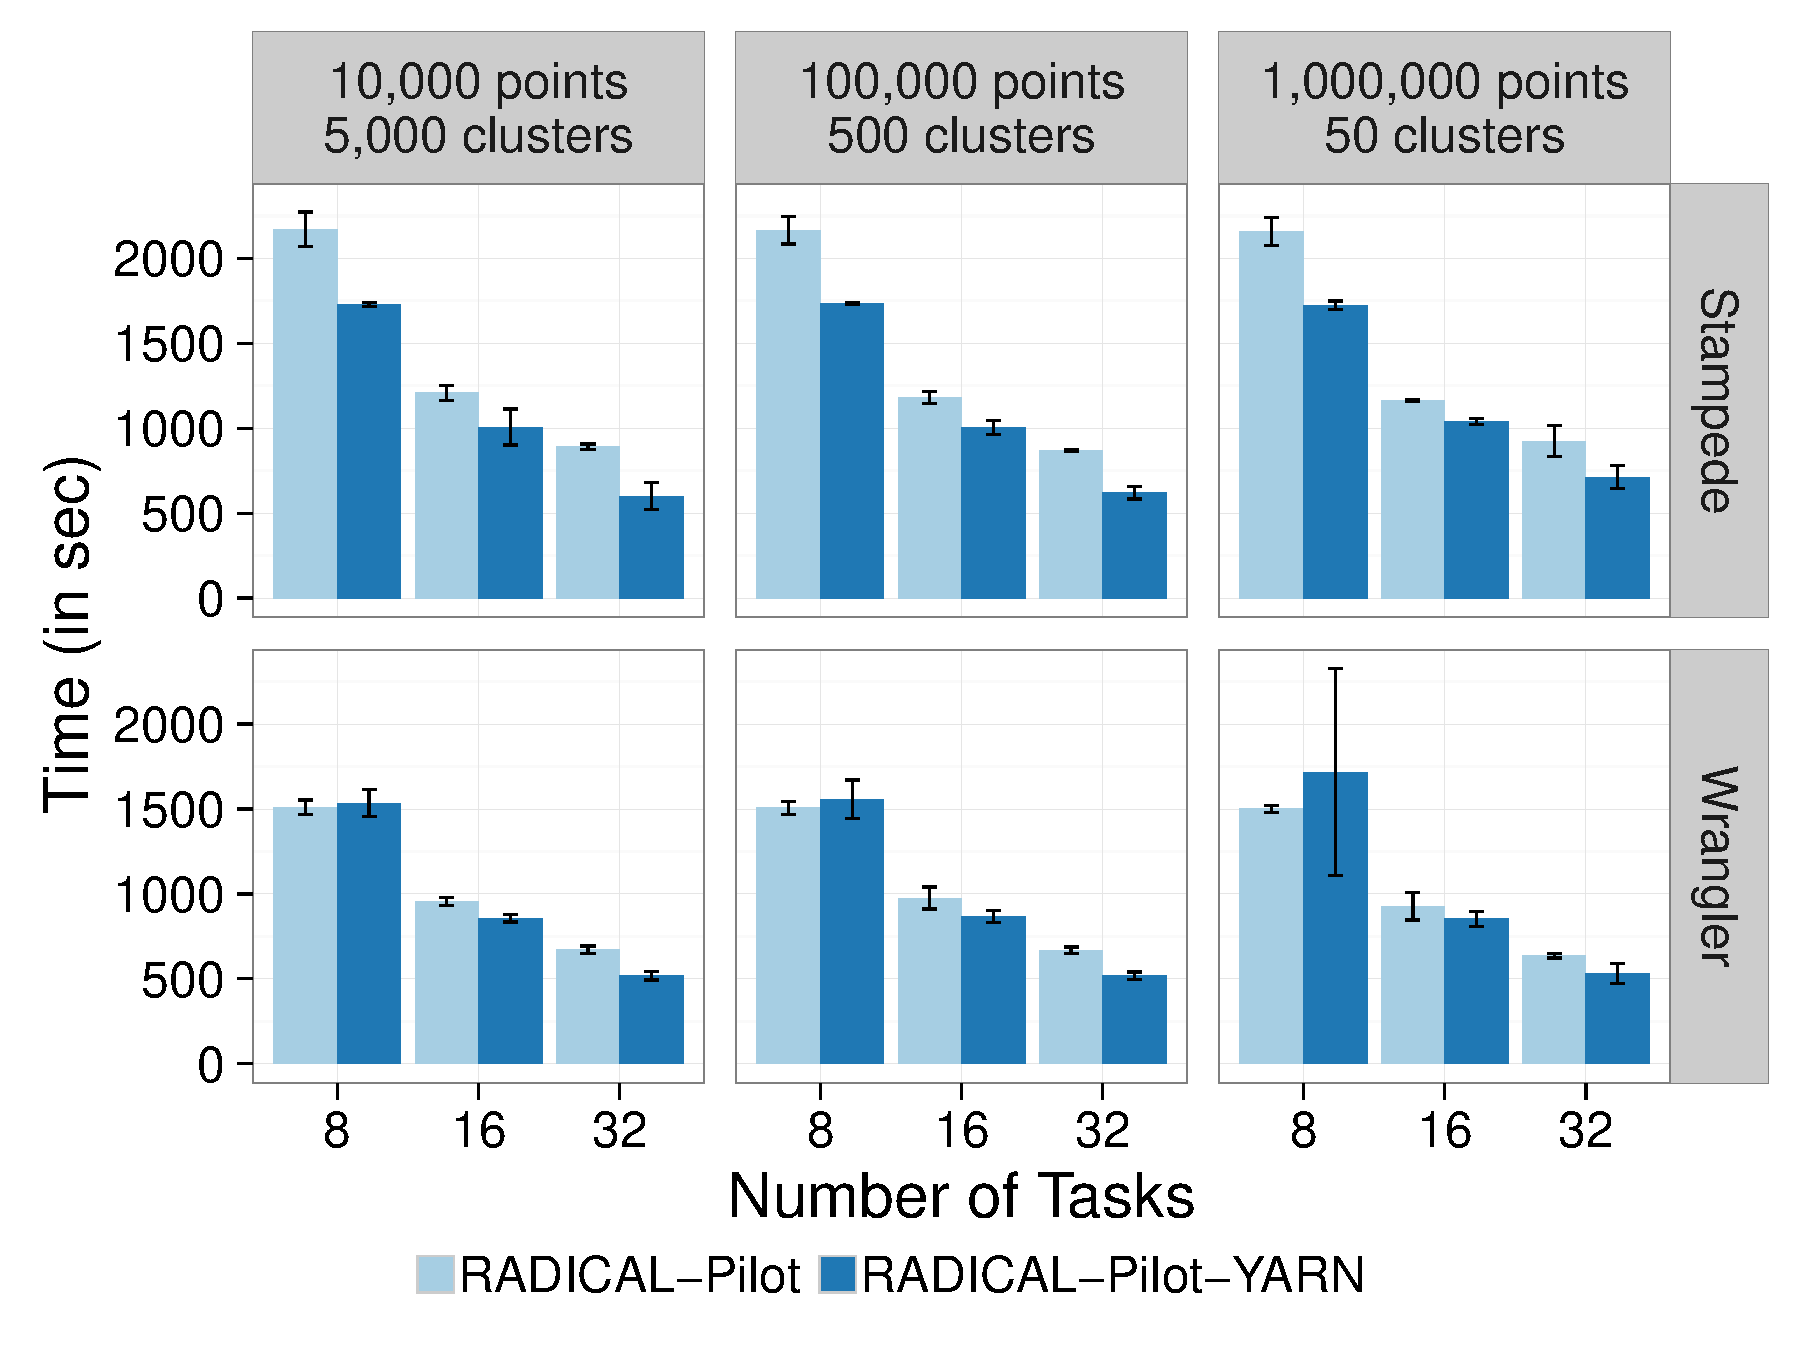
\includegraphics[width=.95\textwidth]{figures/data_analytics_hpc/hpc_hadoop/kmeans.pdf}
    \caption{\textbf{RADICAL~-Pilot and YARN-based K-Means on Stampede and Wrangler:}
        Across all configurations the performance of the YARN backend is in average 13\,\% better.
        On Wrangler a significant better performance and scalability (higher speedups) were observed.}
    \label{fig:experiments_kmeans_rpyarnkmeans}
\end{figure}

Independent of the scenario, the runtimes decrease with the number of tasks.
In particular, in the 8 task scenarios the overhead of YARN is visible.
In particular for larger number of tasks, we observed on average 13\,\% shorter runtimes for RADICAL~-Pilot-YARN.
Also, RADICAL~-Pilot-YARN achieves better speedups, e.\,g., 3.2 for 32 tasks for the 1 million points scenario, which is significantly higher than the RADICAL~-Pilot speedup of 2.4 (both on Wrangler and compared to base case of 8 tasks).
One of the reason for this is that for RADICAL~-Pilot-YARN the local file system is used, while for RADICAL~-Pilot the Lustre filesystem is used.

For similar scenarios and task/resource configuration, the runtimes on Wrangler show a significant performance improvements over Stampede.
This is attributed to the better hardware (CPUs, memory).
In particular for RADICAL~-Pilot-YARN we observed on average higher speedups on Wrangler, indicating that we saturated the 32 GB of memory available on each Stampede node.

In summary, despite the overheads of RADICAL~-Pilot-YARN with respect to Pilot and Compute Unit startup time, we were able to observe performance improvements (on average 13\,\% better time to solution) mainly due to the better performance of the local disks.
